\chapter{Introduction}

Lately, touchless interface devices have appeared in the technology world making our lives easier. Currently the average household pays over 100 dollars a month for electricity according to the U.S. Energy Information Administration. Half of those costs are to keep the motor and compressors in operation in air conditioners and heating systems. If consumers had the ability to control their home’s climate control systems remotely, they could save money without sacrificing convenience and comfort.
The idea is to extend the Kinect's potential uses from gaming to be used in different regions making more and better use of it's capabilities. This is a handicapped-friendly project that provides an easy way to control home devices using Microsoft Kinect sensor and ARDUINO board by giving certain voice commands or by doing certain gestures or even through a touchless graphical interface.


\section{Kinect Features}

The kinect sensor contains of an infrared projector, a LED light indicator, a color camera, an IR camera, a Microphone array and a tilt motor with a vertical range of -27 to 27 degrees.
The camera has an angular field of view of 57 degrees horizontally and 43 degrees vertically.
The connection between the arduino uno board and the kinect sensor is done through a USB-Serial communication.

See \Figref{fig:kinectsensor} (see \figref{fig:kinectsensor})


\begin{figure}[tbp]
  \centering
  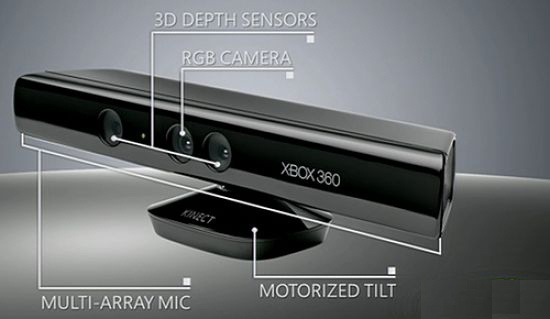
\includegraphics[width=.5\linewidth]{KinectSensor.jpg}
  \caption{Kinect sensor}
  \label{fig:kinectsensor}
\end{figure}
  
\begin{figure}[tp]
  \centering
  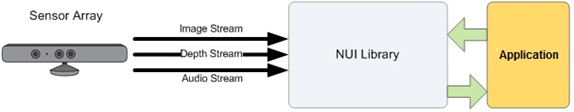
\includegraphics[width=1.0\linewidth]{KinectDataStream.png}
  \caption{Data stream}
  \label{fig:datastream}
\end{figure}
  

\subsection{Skeletal Tracking}

The Microsoft SDK provides the player's skeleton as an array of joints of a Vector4 value each, which contains each joint's x,y,z and w values; it's x,y,z position values in 3d space and the w value that indicates  the quality level (Range between 0-1)) of the position that indicates the center of mass for that skeleton which is only 1 for passive fully tracked players. The kinect sensor can detect up to 6 players at the same time, however it can only track 2 at the same time while it only stores some basic information like position values for the other 4.
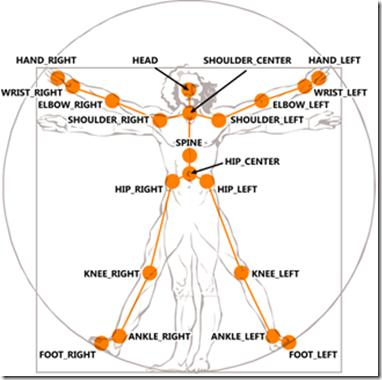
\includegraphics[scale=2]{SkeletonJoints.png}

\subsection{Speech Recognition}

The microphone array of the kinect sensor is responsible for it's hearing, by integrating it's features and creating grammars the kinect can be used for voice recognition.

\subsection{Gesture Recognition}

There's many ways you could build a gesture recognition system using the kinect SDK for example you can store your gestures as frame images and use image proccessing to compare them, or you can just compare the angle between certain joints but this won't be as efficient as it may detect other random gestures too, so it's better to compare joint positions relatively to eachothers or draw imagionary vectors between the joints and compare them to the expected directions. 
You can divide the gesture into smaller gesture parts/segments if needed and check if they succeed in each frame according to their topological order in a certain number of frames then the gesture succeeds.
In this project, the gesture recognition system does all of the above except image proccessing as there was no gesture recording software compatible with the microsoft sdk found.

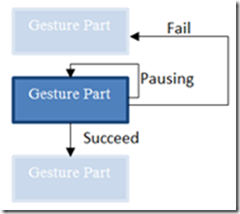
\includegraphics[width=1.0\linewidth]{GestureArchitecture1.png}
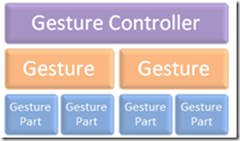
\includegraphics[width=1.0\linewidth]{GestureArchitecture2.png}

\section{Arduino}

The Arduino Uno is a microcontroller board based on the ATmega328 . It has 14 digital input/output pins of which 6 can be used as PWM outputs, 6 analog inputs, a 16 MHz ceramic resonator, a USB connection, a power jack, an ICSP header, and a reset button.
The power pins are as follows:
The ATmega328 has a 32 KB memory (with 0.5 KB used for the bootloader). It also has 2 KB of SRAM and 1 KB of EEPROM.
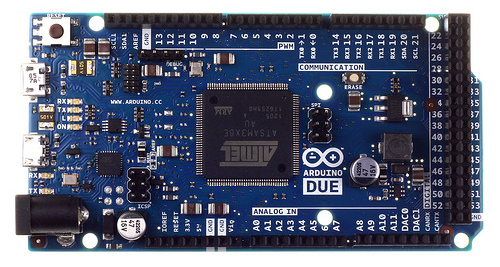
\includegraphics[scale=2]{ArduinoUNOBoard.jpg}

\subsection{Kinect-Arduino-HomeDevice physical Connection}

The connection between the kinect and the arduino is handled through a USB to Serial converter and an interface handling the websockets.
The connection between the arduino and the home devices is made through an electric circuit using sensors, relays, transistors, resistors, LEDS and an LCD etc..
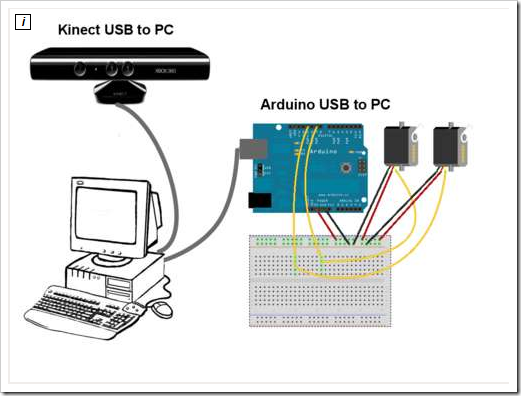
\includegraphics[scale=2]{Kinect-Arduino-Connection.png}

\section{User Stories}

The user stories and the program features are as follows:
\begin{itemize}
\item As a user, I can turn the lights on/off by entering/leaving the room.
\item As a system, I should be able to recognize certain gestures and control the device accordingly.
\item As a user, I can interact with a touchless interface.
\item As a system, I should recognize the user's face and keep track of it.
\item As a user, I can give certain voice commands.
\item As a system, I should have a circuit connection between the arduino board and the device I want to control.
\item As a system, I should be able to control the device and switch it on/off when needed.
\item As a system, I should create an interface to allow the communication between the kinect sensor and arduino board.
\item As  a user, I should see pop-up screens to show feedback from the interface at certain circumstances.
\item As a user, I should see an avatar which represents my distance to the kinect.
\item As a user, I should see an introductory fading screen to the application.
\item As a user, I can play music.
\item As a user, I should see a main screen where I can edit settings and enable/disable features like face/depth/voice/skeletal tracking.
\item As a user, I should see a screen for each controlled device where I can edit it's settings manually.
\item As a system I should provide a way for the user to enter a password to be able to manage the application.
\end{itemize}

\section{Software Architecture}

The software architecture of the project is shown in the figures below
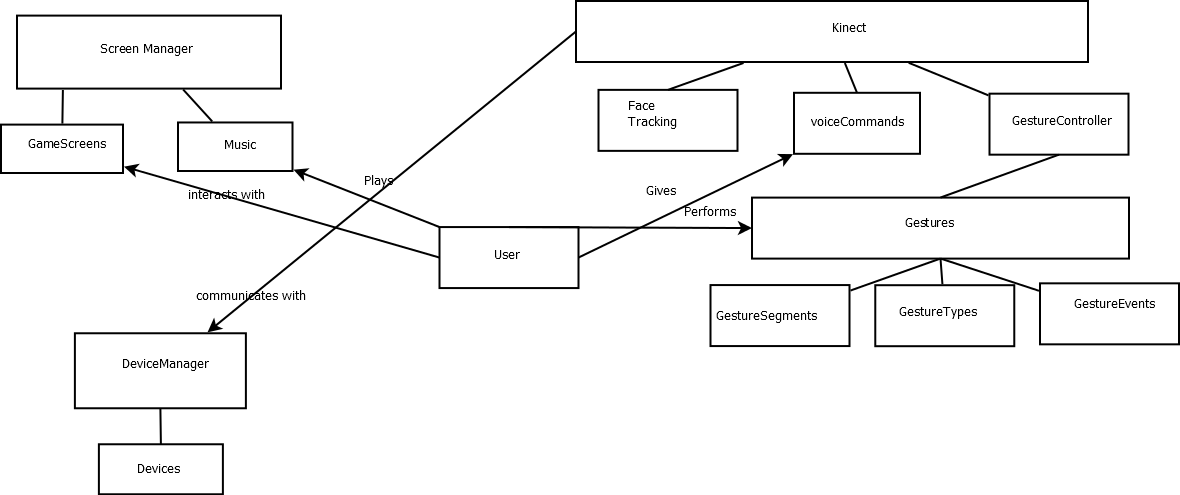
\includegraphics[width=0.8\linewidth]{SoftwareArchitecture}

%%% Local Variables: 
%%% mode: latex
%%% TeX-master: "../Thesis"
%%% End: 
